\chapter*{Приложение В Порядок выполнения лабораторной работы \No3}
\refstepcounter{chapter}
\addcontentsline{toc}{chapter}{Приложение В Порядок выполнения лабораторной работы \No3}
\begin{enumerate}
\item Выбрать вариант задания в приложении \ref{Lab3Var} в соответствии с номером в журнале.
\item Создать в папке с номером группы на рабочем столе папку \verb#Lab3# для файлов проекта.
\item Скопировать в созданную папку \verb#Lab3#, папку  \verb#CMSIS# из папки  \verb#Лабораторные работы по микроконтроллерам/Materials# на рабочем столе.
\item Скопировать в созданную папку \verb#Lab3#, папку  \verb#STM32L1xx_StdPeriph_Driver# из папки  \verb#Лабораторные работы по микроконтроллерам/Materials# на рабочем столе.
\item Скопировать в созданную папку \verb#Lab3#, папку  \verb#STM32_TouchSensing_Drive# из папки  \verb#Лабораторные работы по микроконтроллерам/Materials# на рабочем столе.
\item Скопировать в созданную папку \verb#Lab3#, папку  \verb#Discovery# из папки  \verb#Лабораторные работы по микроконтроллерам/Materials# на рабочем столе.
\item Скопировать в созданную папку \verb#Lab3# файлы \textit{stm32\_tsl\_conf.h, stm32l1xx\_conf.h} из папки  \verb#Лабораторные работы по микроконтроллерам/Materials# на рабочем столе.
\item Создать и настроить проект в среде разработки IAR.
\item В настройках проекта в категории \textit{C/C++ Compiler} во вкладке \textit{Preprocessor} указать путь до всех вложенных папок в папке \verb#Lab3#, заменяя Lab3 на \verb#$PROJ_DIR$# (см. лаб.1).
\item В качестве имени проекта указать \textit{lab3}, все файлы настроек проекта сохранить в папке \verb#Lab3#.
\item Добавить в проект все файлы библиотеки \textit{TSL} (папка \verb#STM32_TouchSensing_Driver#), все файлы из папки \verb#Discovery#.
\item Добавьте в проект файлы \textit{stm32\_tsl\_conf.h, stm32l1xx\_conf.h}.
\item Добавьте в проект файлы \textit{stm32l1xx\_gpio.h, stm32l1xx\_rcc.h, stm32l1xx\_lcd.h, stm32l1xx\_exti.h, stm32l1xx\_gpio.c, stm32l1xx\_rcc.c, stm32l1xx\_lcd.c, stm32l1xx\_exti.c} из \textit{SPL} (папка \verb#STM32L1xx_StdPeriph_Driver#).
\item В добавленные файлы из папки \verb#STM32L1xx_StdPeriph_Driver# добавить
\begin{verbatim}
#include "stm32l1xx_conf.h"
\end{verbatim}
\item Добавить в проект файлы \textit{system\_stm32l1xx.h, system\_stm32l1xx.c, stm32l1xx.h} из папки \verb#Лабораторные работы по микроконтроллерам/#
\verb#Materials/CMSIS/DeviceSupport/ST/STM32L1xx#.
\item Добавьте в проект файл \textit{startup\_stm32l1xx\_md.s} из папки \verb#Лабораторные работы по микроконтроллерам/Materials CMSIS/#
\verb#CM3/DeviceSupport/ST/STM32L1xx/startup/iar#
\item Добавить в проект файлы все файлы из папки \verb#Discovery#
\item Написать программу для микроконтроллера на языке Си.
\item Изменить функции \textit{Button\_value()} и \textit{Slider\_value()}  в файле \textit{discover\_functions.c} в соответствии с вариантом задания.
\item Подключить отладочную плату STM32L - Discovery к компьютеру.
\item Загрузить программу в микроконтроллер и произвести ее отладку. 
\item Составить отчет.
\end{enumerate}

\section{Пример выполнения лабораторной работы \No3}
Разработать программу в среде IAR. Режимы работы периферии приведены в таблице. В первом столбце приведены положения пользовательской кнопки \textit{USER} (количество соответствующих нажатий). Во втором столбце режимы работы сенсорной панели (слайдер или четыре раздельные кнопки). Третий столбец определена информация, выводимая на ЖКИ. Четвертый и пятый столбцы указывают режимы работы для светодиодов.

\begin{figure}[H]
\begin{center}
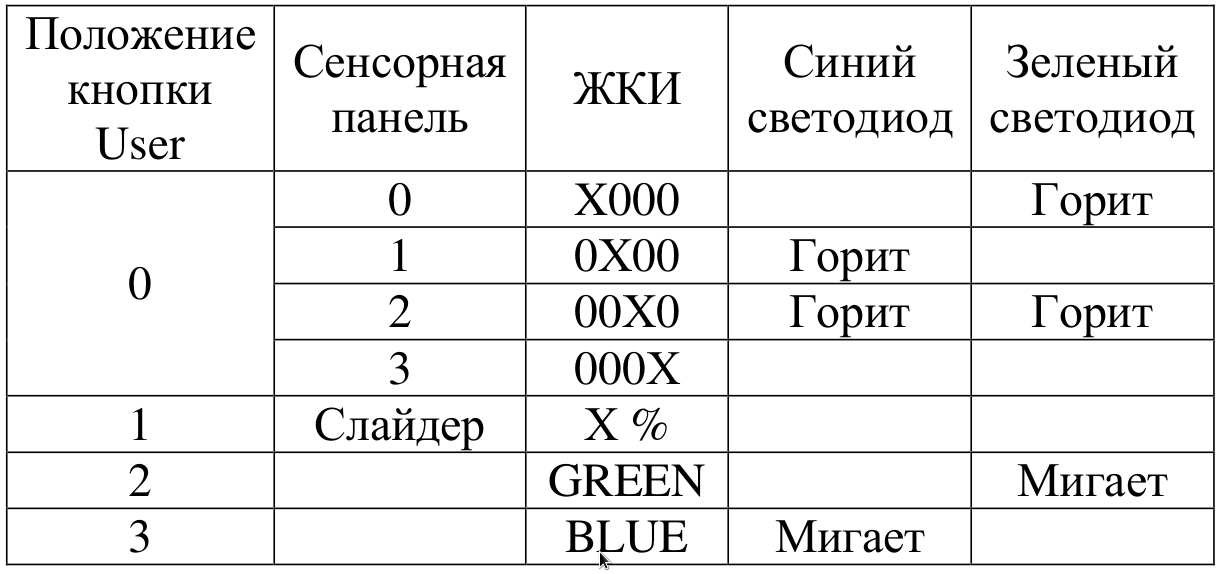
\includegraphics[scale=0.28]{Image/88.jpg} 
\end{center}
\caption{Задание к лабораторной работе}
\end{figure}

\begin{figure}[H]
\begin{center}
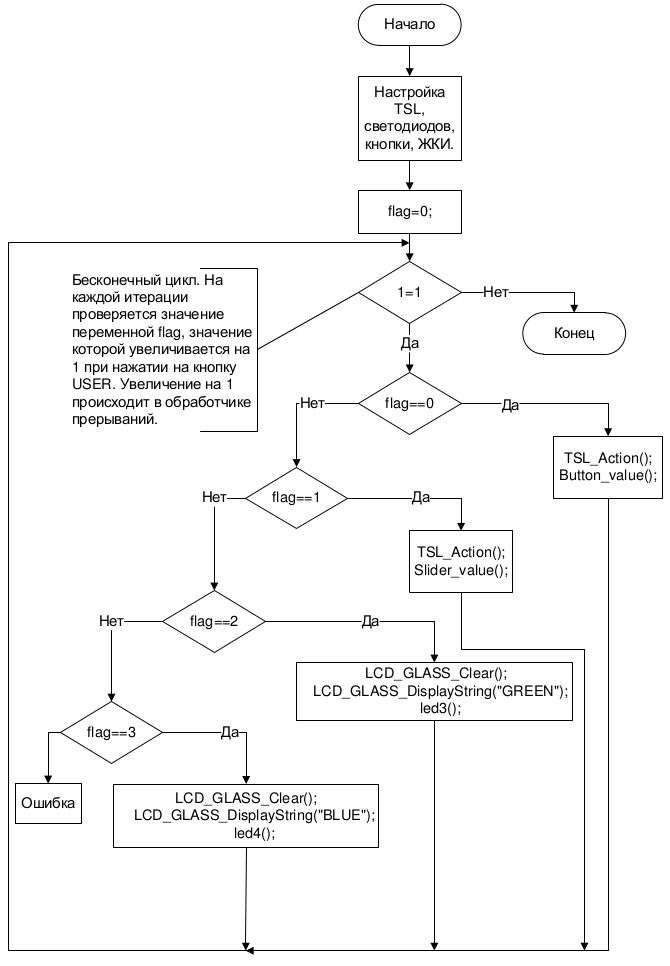
\includegraphics[scale=0.7]{Image/89.jpg} 
\end{center}
\caption{Блок схема алгоритма главной программы}
\end{figure}

\begin{figure}[H]
\begin{center}
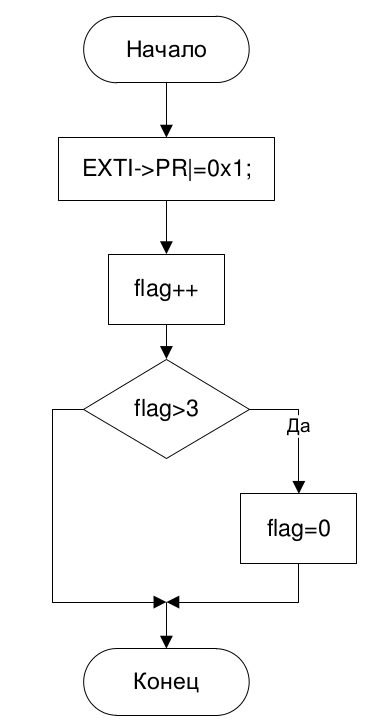
\includegraphics[scale=0.4]{Image/90.jpg} 
\end{center}
\caption{Блок схема алгоритма обработчика прерываний}
\end{figure}

Пример главной программы для микроконтроллера
\begin{verbatim}
#include "stm32l1xx_rcc.h"
#include "stm32l1xx_gpio.h"
//API для работы с TSL
#include "stm32_tsl_api.h"
//Функции для работы с сенсорной панелью 
#include "discover_functions.h"
//Функции для работы с ЖКИ
#include "stm32l_discovery_lcd.h"

/*################ Прототипы функций #############*/
void gpio(void);//Инициализация портов
void controller(void);//Инициализация контроллера ЖКИ
void delay(uint32_t); //Временная задержка в миллисекундах
void led3(void);
void led4(void);
void handler(void);//Обработчик прерываний

//Значение переменной flag меняется в обработчике 
//прерываний EXTI0_IRQHandler() при нажатия кнопки
int flag=0;
static uint32_t TimingDelay;


void main(void)
{
    /*############ Настройка светодиодов #############*/ 
     GPIO_InitTypeDef GPIO_InitStructure;
    //Включение тактирования
    RCC_AHBPeriphClockCmd(RCC_AHBPeriph_GPIOB, ENABLE);
    GPIO_InitStructure.GPIO_Pin = GPIO_Pin_7 | GPIO_Pin_6 ;
    GPIO_InitStructure.GPIO_Mode = GPIO_Mode_OUT;
    GPIO_InitStructure.GPIO_Speed = GPIO_Speed_400KHz;
    GPIO_InitStructure.GPIO_OType = GPIO_OType_PP;
    //Инициализация структуры
    GPIO_Init(GPIOB, &GPIO_InitStructure);
    
    /*################ Настройка прерываний #############*/ 
    EXTI->IMR|=EXTI_IMR_MR0;                          
    EXTI->RTSR|=EXTI_RTSR_TR0;                          
    NVIC_EnableIRQ (EXTI0_IRQn); 
        
    /*###### Настройка GPIO и контроллера ЖКИ ######*/   
    gpio();
    controller();
    
    /*################ Настройка кнопки USER #############*/ 
    GPIO_InitStructure.GPIO_Pin = GPIO_Pin_0;
    GPIO_InitStructure.GPIO_Mode = GPIO_Mode_IN;
    GPIO_InitStructure.GPIO_PuPd = GPIO_PuPd_NOPULL;//ВАЖНО!
    GPIO_InitStructure.GPIO_Speed = GPIO_Speed_40MHz;
    GPIO_Init(GPIOA, &GPIO_InitStructure);
    
    /*############# Настройка сенсорной панели #############*/ 
    TSL_Init();
    sMCKeyInfo[0].Setting.b.IMPLEMENTED = 1;
    sMCKeyInfo[0].Setting.b.ENABLED = 1;
    sMCKeyInfo[0].DxSGroup = 0x00; 
    
    /*######### Главная программа в бесконечном цикле ######*/  
      while(1)
      {
          if (flag==0)
          {
                TSL_Action();
                Button_value();//Сенсорная панель как 4 раздельные кнопки
          } 
          else if (flag==1)
          {
                TSL_Action();
                Slider_value();//Сенсорная панель как слайдер
          } 
          else if (flag==2)
          {
            
               LCD_GLASS_Clear();//Очистили ЖКИ
               LCD_GLASS_DisplayString("GREEN");//Вывели на ЖКИ GREEN
               led3();//Мигаем зеленым светодиодом
          }
          else if (flag==3)
          {
                LCD_GLASS_Clear();//Очистили ЖКИ
                LCD_GLASS_DisplayString("BLUE");//Вывели на ЖКИ BLUE
                led4();//Мигаем синим светодиодом
          } 
      }
}
/*##### Тактирование контроллера ЖКИ и сенсорной панели #####*/ 
void controller(void)
{
/*################ Тактирование HSI #############*/ 
    RCC->CR |=0x1;
    while(!(RCC->CR&RCC_CR_HSIRDY));
    RCC->CFGR |=0x1; 

/*################ Тактирование контроллера ЖКИ #############*/   
    RCC->APB1ENR |= 0x90000200; //плюс тактирование 
                                  компаратора в 31 разряде
    PWR->CR |= 0x100;
    RCC->CSR |= 0x800000;
    RCC->CSR &= ~0x800000;
    RCC->CSR |= 0x100;
    while(!(RCC->CSR&RCC_CSR_LSERDY));
    RCC->CSR |= 0x10000;
    LCD->CR &= ~0x60;
    LCD->CR |= 0x40;
    LCD->CR &= ~0x1C;
    LCD->CR |= 0xC;
    LCD->CR |= 0x80;
    LCD->FCR &= ~0x3C00000;
    LCD->FCR &= ~0x3C0000;
    LCD->FCR |= 0x40000; //ps=1 div=17
    LCD->FCR &= ~0x1C00;
    LCD->FCR |= 0x800;
    while(!(LCD->SR&LCD_SR_FCRSR));
    LCD->CR &= ~0x2;
    LCD->CR |= 0x1;
    while(!(LCD->SR&LCD_SR_RDY));
    while(!(LCD->SR&LCD_SR_ENS));
}
/*########## Настройка портов GPIO для работы с ЖКИ ##########*/ 
void gpio(void)
{
    RCC->AHBENR |= 0x7;
    GPIOA->MODER |= 0x802A00A8;
    GPIOB->MODER |= 0xAAAA0A80;
    GPIOC->MODER |= 0xAAA0AA;
    GPIOA->OTYPER &= ~0x870E;
    GPIOB->OTYPER &= ~0xFF38;
    GPIOC->OTYPER &= ~0xFCF;
    GPIOA->PUPDR &= ~0xC03F00FC;
    GPIOB->PUPDR &= ~0xFFFF0FC0;
    GPIOC->PUPDR &= ~0xFFF0FF;
    GPIOA->OSPEEDR &= ~0xC03F00FC;
    GPIOB->OSPEEDR &= ~0xFFFF0FC0;
    GPIOC->OSPEEDR &= ~0xFFFFF0FF;
    GPIOA->AFR[0] |= 0xBBB0;
    GPIOA->AFR[1] |= 0xB0000BBB;
    GPIOB->AFR[0] |= 0xBBB000;
    GPIOB->AFR[1] |= 0xBBBBBBBB;
    GPIOC->AFR[0] |= 0xBB00BBBB;
    GPIOC->AFR[1] |= 0xBBBB;
}
/*############# Функция задержки в миллисекундах ##########*/
void delay(uint32_t nTime)//Определение функции delay()
{
  TimingDelay = nTime;
  while(TimingDelay != 0);
}

/*################ Мигание зеленым светодиодом #############*/
void led3(void) //Определение функции led3()
{
    GPIO_SetBits(GPIOB, GPIO_Pin_7);
    delay(250);//250 мс
    GPIO_ResetBits(GPIOB, GPIO_Pin_7);
    delay(250);
}
/*################ Мигание синим светодиодом #############*/
void led4(void) //Определение функции led4()
{
    GPIO_SetBits(GPIOB, GPIO_Pin_6);
    delay(250);
    GPIO_ResetBits(GPIOB, GPIO_Pin_6);
    delay(250);
}
/*################ Обработчик прерываний #############*/ 
//Обработчик прерывания нажатия на кнопку
void EXTI0_IRQHandler(void)
{
      EXTI->PR|=0x01; //Сброс бита события, вызвавшего прерывание
      flag++;
      if (flag>3)
        flag=0;
}

//Обработчик прерывания системного таймера
//Вызов функции SysTick_Config() определенной в core_cm3.h 
//происходит в файле stm32_tsl_timebase.c
void SysTick_Handler(void)
{    
  if (TimingDelay != 0x00)
  {
    TimingDelay--;
  }
}
\end{verbatim}
Пример изменения файла \textit{discover\_functions.c}
\begin{verbatim}
/*########## Вывод точки касания в процентах #############*/  
void Slider_value(void)
{
  uint16_t Message[6];  
  uint32_t percent_value;
/*################ Отключили светодиоды #############*/  
  GPIO_ResetBits(GPIOB, GPIO_Pin_6);
  GPIO_ResetBits(GPIOB, GPIO_Pin_7);
 
/*В массив Massage[] заносятся символы для отображения на ЖКИ */ 
  Message[0] = ' ';
  Message[1] = ' ';
  Message[2] = ' ';

  if ((TSL_GlobalSetting.b.CHANGED) && (TSLState == TSL_IDLE_STATE)) 
  {
    TSL_GlobalSetting.b.CHANGED = 0;
  }//Если касание обнаружено
  if ((SLIDER_DETECTED)&&(TSLState == TSL_IDLE_STATE))  {
/*###### Вычисление положения касания сенсорной панели #####*/ 
    percent_value = SLIDER_POSITION ;
    percent_value *= 10000;
    percent_value /= 255 ;
/*##### Функция перевода значения в char #####*/      
    convert_into_char(percent_value,Message);
    Message[3] = '°' ;
    Message[4] = '/' ;
    Message[5] = '%' ;   
/* Вывод на ЖКИ в виде "X %", где Х - положение точки касания */
    LCD_GLASS_DisplayStrDeci(Message);
  } 
  else if((!TSL_GlobalSetting.b.CHANGED) && (TSLState == TSL_IDLE_STATE))
  {     //Если касание не обнаружено
        Message[3] = '°' ;
        Message[4] = '/' ;
        Message[5] = '%' ;   
        LCD_GLASS_DisplayStrDeci(Message);
  } 
}/*###########################################################*/  

/*####### Сенсорная панель как 4 раздельные кнопки ########*/  
void Button_value(void)
{
  uint8_t Message[6];  
/*В массив Massage[] заносятся символы для отображения на ЖКИ */   
    Message[0] = ' ';
    Message[1] = '0';
    Message[2] = '0';
    Message[3] = '0';
    Message[4] = '0';
    Message[5] = ' ';
    
  if ((TSL_GlobalSetting.b.CHANGED) && (TSLState == TSL_IDLE_STATE)) 
  {
    TSL_GlobalSetting.b.CHANGED = 0;

  }//Если касание обнаружено
  if ((SLIDER_DETECTED)&&(TSLState == TSL_IDLE_STATE))  {
/*Вся область сенсорной панели делится на 
  4 части определением точки касания*/  
    if( SLIDER_POSITION <= 25 ){
      Message[1] = 255;       
      GPIO_SetBits(GPIOB, GPIO_Pin_7); //Включили зеленый светодиод
      GPIO_ResetBits(GPIOB, GPIO_Pin_6);} //Отключили синий светодиод

    if( (SLIDER_POSITION > 25 ) && (SLIDER_POSITION <= 110 )) {       
      Message[2] = 255; 
      GPIO_ResetBits(GPIOB, GPIO_Pin_7); //Отключили зеленый светодиод
      GPIO_SetBits(GPIOB, GPIO_Pin_6);  } //Включили синий светодиод
    if( (SLIDER_POSITION > 110 ) && (SLIDER_POSITION <= 200 ))  {      
      Message[3] = 255;  
      GPIO_SetBits(GPIOB, GPIO_Pin_6);  //Включили синий светодиод
      GPIO_SetBits(GPIOB, GPIO_Pin_7); }//Включили зеленый светодиод
      
    if( SLIDER_POSITION > 200 )    {    
      Message[4] = 255;
      GPIO_ResetBits(GPIOB, GPIO_Pin_6); //Отключили синий светодиод
      GPIO_ResetBits(GPIOB, GPIO_Pin_7);}//Отключ. зеленый светодиод
      
/*Вывод на ЖКИ в виде "0Х00", где Х - положение точки касания */   
   LCD_GLASS_DisplayString(Message);
  } 
  else if((!TSL_GlobalSetting.b.CHANGED) &&
   (TSLState == TSL_IDLE_STATE))
  {     //Если касание не обнаружено
        LCD_GLASS_DisplayString(Message);
  }
   
}
\end{verbatim}


\section{Варианты заданий к лабораторной работе \No3}
\label{Lab3Var}
\begin{figure}[H]
\begin{center}
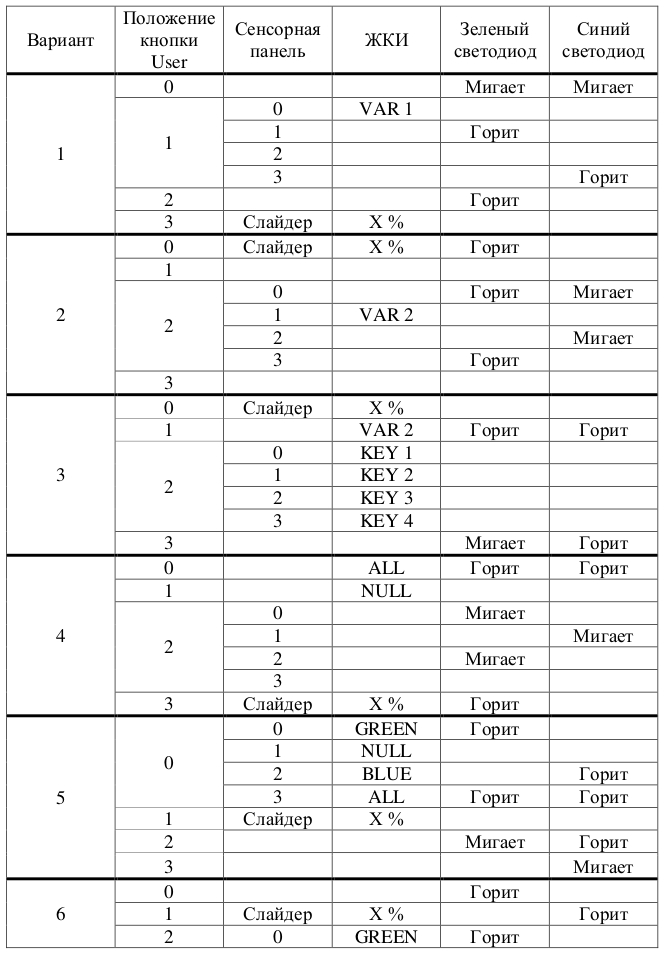
\includegraphics[scale=0.7]{Image/91.jpg} 
\end{center}
\end{figure}


\begin{figure}[H]
\begin{center}
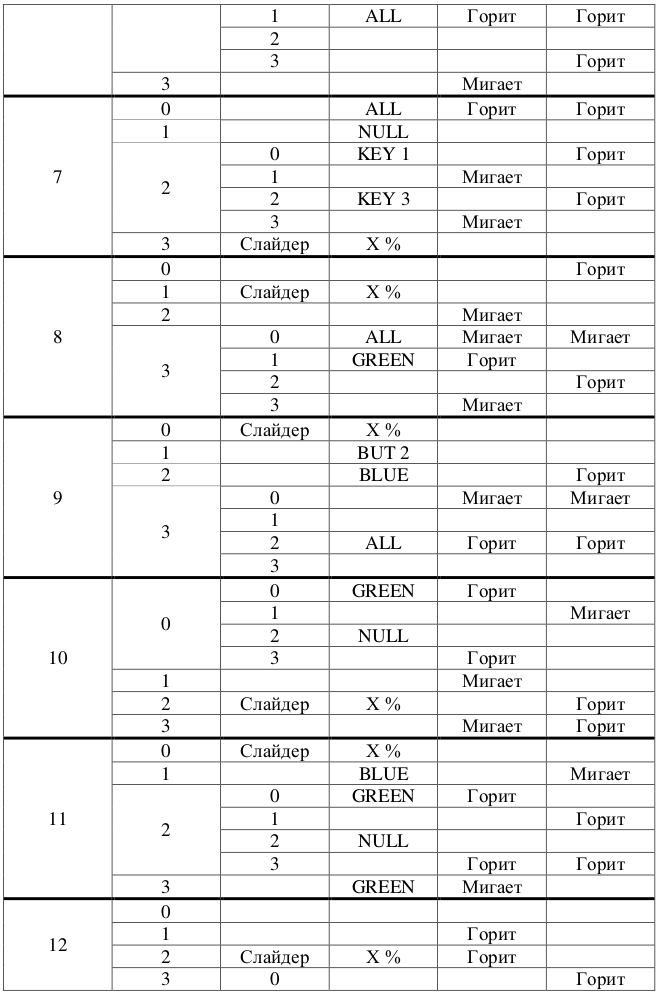
\includegraphics[scale=0.7]{Image/92.jpg} 
\end{center}
\end{figure}

\begin{figure}[H]
\begin{center}
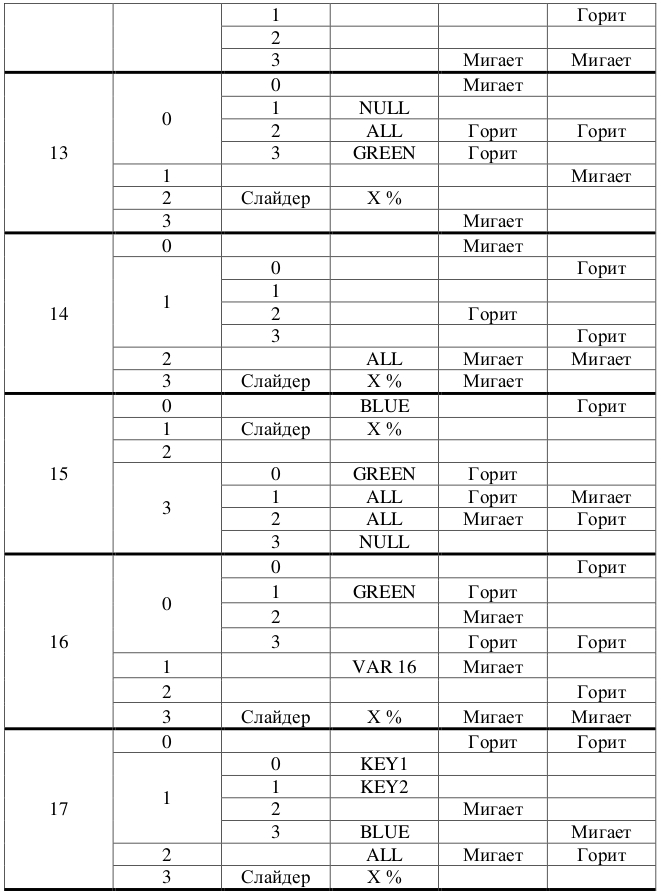
\includegraphics[scale=0.7]{Image/93.jpg} 
\end{center}
\end{figure}